%!TEX program = xelatex
\documentclass[cn,hazy,blue,14pt,screen]{./cls/elegantnote}
\title{Euler-Lagrange Equation}

\author{Yongchao Zhang}
\institute{NORTHWEST UNIVERSITY}

%\version{2.30}
%\date{\zhtoday}
\date{\today}

% --- my format --- %

%---------------------------%
%------- paper settings -------%
%\textwidth 17cm
%\textheight 24cm
%\hoffset -20mm
%\voffset -20mm

%------- figures settings -------%
\graphicspath{./figures}



%-----------------------------%
%------- bibliographystyle -------%
%% Numbered
%\bibliographystyle{model1-num-names}

%% Numbered without titles
%\bibliographystyle{model1a-num-names}

%% Harvard
%\bibliographystyle{model2-names.bst}\biboptions{authoryear}

%% Vancouver numbered
%\usepackage{numcompress}\bibliographystyle{model3-num-names}

%% Vancouver name/year
%\usepackage{numcompress}\bibliographystyle{model4-names}\biboptions{authoryear}

%% APA style
%\bibliographystyle{model5-names}\biboptions{authoryear}

%% AMA style
%\usepackage{numcompress}\bibliographystyle{model6-num-names}
\bibliographystyle{./cls/elsarticle-num}
% --- my packages --- %

%-----------------------------%
%------- package settings -------%
\usepackage{amsmath,amssymb,amsthm}
\allowdisplaybreaks[4]  %  放在 amsmath 之后. 允许公式跨页, 1,2,3,4 代表执行跨页强度. 4最强. 
\usepackage{hyperref}
\usepackage{cleveref}
\usepackage{graphicx}
\usepackage{graphics}
\usepackage {graphicx,fancyhdr}
\usepackage{graphics}
\usepackage{color}
\usepackage{flafter}
\usepackage{multirow}
\usepackage{mathrsfs} % 花体
\usepackage{subfigure}
\usepackage{tabularx}
\usepackage{lineno}
\usepackage{xfrac}
\usepackage{rotating} % Rotating table
\usepackage{stmaryrd} % contain jump [[ ]], bing `latex stmaryrd` to see more usage.
\usepackage{bm} % 粗斜体
\usepackage{cases} % for the begin{numcases} ... end{cases}
\usepackage{enumerate}
\usepackage{ulem}  % 删除线相关的 package: \sout{文字} %删除线; \uwave{文字} %波浪线; \xout{文字} %斜删除线; \uuline{文字}  %双下划线

%---------------------------%
%------- other settings -------%
% 下面两个必须放在 \usepackage{...} 后面
%\numberwithin{equation}{section}  % 公式随章节自动编号
\modulolinenumbers[5]  % 指定每隔 5 行显示行号

% --- my command --- %

%----------------------------------%
%------- define new commmads -------%
\newcommand*{\snorm}[1]{\lvert #1 \rvert} % the seminorm norm: |..|
\newcommand*{\dnorm}[1]{\lVert #1\rVert} % the double norm: ||..||
\newcommand*{\tnorm}[1]{\interleave#1\interleave} % the triple norm: |||..|||
\newcommand*{\anglebrackets}[1]{\langle#1\rangle} % the angle brackets: <...>
\newcommand*{\jump}[1]{\llbracket #1\rrbracket} % the vector jump brackets: [[...]]
\newcommand*{\hhoVecvars}[1]{\underline{\bm{#1}}}
\newcommand*{\hhoScalvars}[1]{\underline{{#1}}}
\newcommand*{\hhonormalvec}[1]{ \bm{n}_{_{#1} } }
\newcommand*{\divOperator}[1]{\text{\rm{div} \hspace{-0.5mm}}{#1}}
\newcommand*{\DivOperator}[1]{\text{\rm{div} \hspace{-0.5mm}}{#1}}
\newcommand*{\divtau}[1]{\text{div$ _{\tau} $ \hspace{-0.5mm}}{#1}}
\newcommand*{\divVecOperator}[1]{\text{\textbf{div} \hspace{-0.5mm}}{#1}}
\newcommand*{\DivOperatorVec}[1]{\text{\textbf{div} \hspace{-0.5mm}}{#1}}
\newcommand{\transpose}{\intercal} % the transpose sign
\newcommand{\realR}{\ensuremath{\mathbb{R}}}
\newcommand{\rd}{\ensuremath{\mathbb{R}^d}}
\newcommand{\gd}{d}  % grid dimension
\newcommand{\dx}{\ensuremath{{\,\hspace{-0.06em}\rm{d}}\bm{x}}}
\newcommand{\ds}{\ensuremath{{\,\hspace{-0.06em}\rm{d}}s}}
\newcommand{\littlequad}{\ensuremath{\,\hspace{-0.08em}}}
\newcommand{\sqd}[1]{\ensuremath{[{#1}]^d}}  % [square brackets]^d
\newcommand{\mcalTh}{\mathcal{T}_h}
\newcommand{\mcalFh}{\mathcal{F}_h}
\newcommand{\mcalT}{\mathcal{T}}
\newcommand{\mcalF}{\mathcal{F}}
\newcommand{\mbbP}{\mathbb{P}}
\newcommand{\matvar}[1]{\ensuremath{\uuline{\bm{#1}}}}
\newcommand{\botimes}{\ensuremath{\bm{\otimes}}}
\newcommand{\bcurl}{\ensuremath{{\bf{curl}\hspace{0.1em}}}}
\newcommand{\identityM}{\ensuremath{{\bf{I}}}}
\newcommand{\bdeltaT}{\ensuremath{\bm{\delta}_T^k}}
\newcommand{\bdeltaF}{\ensuremath{\bm{\delta}_{TF}^k}}
\newcommand{\comment}[1]{\iffalse #1 \fi } 


%%--- amsmath - therorm style 
%\theoremstyle{plain}
%\newtheorem{lemma}{Lemma}
%\newtheorem{Theorem}{Theorem}[section]
%\newtheorem{Lemma}[Theorem]{Lemma}
%\newtheorem{Def}[Theorem]{Definition}
%\newtheorem{Remark}[Theorem]{Remark}
%\newtheorem{Exam}{Example}{\normalfont}
%\newtheorem*{Proof}{Proof} % there is no number behind the proof.


%%------- re-define 
\renewcommand\arraystretch{1.1}
\renewcommand\proofname{\rm{\textbf{Proof.}}}

\begin{document}

\maketitle

%\centerline{ 
\includegraphics[width=0.2\textwidth]{logo-blue.png} }

\section{Euler-Lagrange Equation}
参考: \href{https://blog.csdn.net/zhongyuchen/article/details/72820909}{欧拉-拉格朗日方程}, 以及 \href{https://www.cnblogs.com/bigmonkey/p/9519387.html}{寻找最好 (2) -- 欧拉-拉格朗日方程}

\rule[1pt]{14.3cm}{0.05em}

欧拉-拉格朗日方程 (Euler-Lagrange equation) 为变分法中的一条重要方程. 它提供了求泛函的平稳值的一个方法, 其最初的想法是初等微积分理论中的 ``可导的极值点一定是稳定点 (临界点)”. 当能量泛函包含微分时, 用变分方法推导其证明过程, 简单地说, 假设当前的函数 (即真实解) 已知, 那么这个解必然使能量泛函取全局最小值.

\subsection{泛函}
我们很清楚函数的概念, 它大致是, 将一个自变量扔到一个黑盒里,  经过黑盒的暗箱操作, 最终得到了一个因变量:
\begin{equation*}
 	x \rightarrow \boxed{f} \rightarrow \mathbb{R}, 
\end{equation*}
泛函是将一个函数作为自变量, 经过黑盒, 最终得到一个实数的因变量:
\begin{align*}
 	f(x) \rightarrow \boxed{L} \rightarrow \mathbb{R},
\end{align*}
可以说, 泛函就是函数的函数, 是更广泛意义上的函数.

\subsection{欧拉-拉格朗日方程}
\subsubsection{最速降线}
有一种泛函称为简单泛函, 如下所示:
\begin{align*}
 	&\mathcal{A}[f] = \int_{x_1}^{x_2} L(x, f(x),f'(x)),\\
 	&f(x)\rightarrow \boxed{\mathcal{A}[f]}\rightarrow \mathbb{R},
\end{align*}
其中 $ L $ 是一个确定的函数, 之所以叫简单函数, 是因为只传递了三个参数, 复杂一点的话还可以继续传递 $ f $ 的高阶导数. 现在的问题是, 如果 $ \mathcal{A} $ 处于极值点, 它对应的 $ f(x) $ 是什么?

这实际上是求一个具体函数, 使得泛函能够取得极值. 一个典型的例子是最速降线问题: 从所有连接不在同一个铅垂线上的定点 $ A $、$ B $ 的曲线中找出一条曲线, 使得初始速度为 $ 0 $ 的质点, 受重力作用, 由 $ A $ 沿着曲线滑下时以最短的时间到达 $ B $, 如图 \ref{fig1}:
\begin{figure}[!htbp]
	\centering
	\caption{$ A $ 到 $ B $.}
	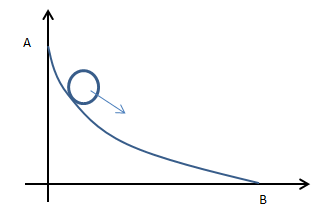
\includegraphics[width=0.4\textwidth]{./figures/1.png}
	\label{fig1}
\end{figure}

这里我们将曲线看作路径 $ f $ 关于时间 $ t $ 的函数, 如图 \ref{fig2}, 
\begin{figure}[!htbp]
	\centering
	\caption{$ f $ 关于时间 $ t $ 的函数}
	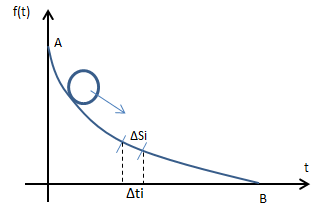
\includegraphics[width=0.4\textwidth]{./figures/2.png}
	\label{fig2}
\end{figure}

其中 $ \Delta S_i $ 是在极短时间 $ \Delta t_i $ 内沿着曲线移动的微小弧长, 此时的瞬时速度是 $ \Delta V_i $, 距离=速度$ \times $时间:
\begin{align*}
	\Delta S_i \approx \Delta V_i \Delta t_i, \quad \Delta t_i \approx \frac{\Delta S_i}{\Delta V_i},
\end{align*}
重力加速的推论, 在 $ t $ 时间处的速度 $ V^2 = 2gh $:
\begin{align*}
 	\Delta t_i \approx \frac{\Delta S_i}{\Delta V_i} = \frac{\Delta S_i}{\sqrt{2gf(t_i)}},
\end{align*}
质点从 $ A $ 点到 $ B $ 点的总时间:
\begin{align*}
 	T&\approx \sum_{i=1}^{n}\frac{\Delta S_i}{\Delta V_i}\sum_{i=1}^{n}\frac{\Delta S_i}{\sqrt{2gf(t_i)}} \\
 	&= \int_{t_A}^{t_B}\frac{dS}{\sqrt{2gf(t)}} dt.
\end{align*}
根据弧长公式, 可以将 $ dS $ 化简, 进一步写成 (关于弧长公式, 可参考: \href{https://www.cnblogs.com/bigmonkey/p/7908854.html}{数学笔记25--弧长和曲面面积}): 
\begin{align*}
 	ds = \int_a^b\sqrt{1+(\frac{dy}{dx})^2} dx = \int_a^b\sqrt{1+(y')^2}dx,
\end{align*}
因此
\begin{align*}
 	T = \int_{t_A}^{t_B}\frac{dS}{\sqrt{2gf(t)}} dt = \int_{t_A}^{t_B}\frac{\sqrt{1+f'(t)^2}}{\sqrt{2gf(t)}} dt.
\end{align*}

把结论和简单泛函做个对比, 可以看到二者形式相吻合:
\begin{align*}
 	&\mathcal{A}[f] = \int_{x_1}^{x_2} L(x,f(x),f'(x)) dx, \\
 	&T[f] =  \int_{t_A}^{t_B}\frac{\sqrt{1+f'(t)^2}}{\sqrt{2gf(t)}} dt, \\
 	&T[f]\rightarrow \mathcal{A}[f], \quad t\rightarrow x, \quad \frac{\sqrt{1+f'(t)^2}}{\sqrt{2gf(t)}} \rightarrow L(x,f(x),f'(x)).
\end{align*}

现在回到最初的问题, $ AB $ 间有无数条曲线, 每条曲线都可以求得时间 $ f(t) $, 在众多的曲线中, 有一条唯一的曲线能够使得 $ T[f] $ 取得最小值, 这个 $ f(t) $ 应该长成什么样?

\subsubsection{EL 方程的推导}
这里先抛开具体的速降问题, 只看 $ \mathcal{A}[f] $, 并且假设 $ f_0(x) $ 就是符合条件的最优函数. 现在, 将 $ f_0(x)+k(x) $ 定义为是有别于最优曲线 $ f_0(x) $ 的其它函数, 其中 $ k(x) $ 可以是任意函数. 如果如下定义 $ f(x, k) $:
\begin{align*}
 	f(x,k)=(f_0+k)(x), \quad f'(x,k)=(f_0+k)'(x).
\end{align*}

因为 $ f_0(x) $ 是最优函数, 此时 $ \mathcal{A}[f_0] $ 有最小值, 则一定有:
\begin{align*}
 	\mathcal{A}[f(x,k)] &\geq \mathcal{A}[f_0], \\
 	\int_{x_1}^{x_2}L(x,f(x,k),f'(x))dx &\geq \int_{x_1}^{x_2}L(x,f_0(x),f_0'(x))dx.
\end{align*}
由于任意函数 $ k(x) $ 不好定义, 为了能够使 $ k(x) $ 任意小, 令:
\begin{align*}
 	k(x) = \epsilon \eta(x) \quad \forall \ \epsilon\in\mathbb{R},
\end{align*}
其中, $ \eta $ 是任意函数, 当 $ \epsilon $ 取极小值时, 可以看作是对 $ f_0(x) $ 的轻微扰动; 还需要额外定义的是, 在端点处是不能扰动的, 即 $ \epsilon \eta(A)=\epsilon \eta(B)=0 $, 这对于任意 $ \epsilon $ 都适用, 所以 $  \eta(A)= \eta(B)=0 $, 如图 \ref{fig3}. 注意 $ \epsilon $ 是对 $ f_0(x) $ 的扰动程度, $ \epsilon \eta(x) $ 是扰动后的增量, $ \epsilon \eta(x)=0 $ 说明扰动为 0, 也就是无扰动, $ f_0(x)+\epsilon \eta(x) $ 才是扰动后的函数.
\begin{figure}[!htbp]
	\centering
	\caption{$ f $ 关于时间 $ x $ 的函数}
	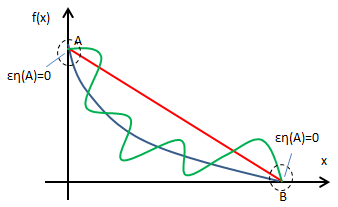
\includegraphics[width=0.4\textwidth]{./figures/3.png}
	\label{fig3}
\end{figure}

由于假设 $ f_0(x) $ 是最优函数, 所以可以将 $ f_0(x) $ 看作已经确定的函数, 如果再将任意函数 $ \eta(x) $ 看作一个确定的函数, 那么 $ \mathcal{A} $ 可以看成 $ \epsilon $ 的函数, 若 $ \mathcal{A}' = 0 $, 函数存在极值, 这已经变成了极值点的求解:
\begin{align*}
 	&f(x,\epsilon) = (f_0+\epsilon\eta)(x), \quad f'(x,\epsilon) = (f_0+\epsilon\eta)'(x), \\
 	&\mathcal{A}[\epsilon] = \int_{x_A}^{x_B}L(x,(f_0+\epsilon\eta)(x), (f_0+\epsilon\eta)'(x) )dx = \int_{x_A}^{x_B} L(x,f(x,\epsilon),f'(x,\epsilon))dx.
\end{align*}

根据链式法则 (可参考\href{https://www.cnblogs.com/bigmonkey/p/8350943.html}{多变量微积分笔记4--全微分与链式法则}):
\begin{align*}
 	&\text{if }\ f = f(x,y,z), \ x=x(t), \ y = y(t), \ z=z(t), \\
 	&\text{then }\ \frac{df}{dt} = \frac{\partial f}{\partial x} \frac{\partial x}{\partial t} +  \frac{\partial f}{\partial y} \frac{\partial y}{\partial t} +  \frac{\partial f}{\partial z} \frac{\partial z}{\partial t}, \\
 	&\text{hence, } \\
 	&\frac{d\mathcal{A}}{d\epsilon} = \int_{x_A}^{x_B} \frac{dL}{d\epsilon} dx = \int_{x_A}^{x_B} \frac{\partial L}{\partial x} \underset{=\,0}{\underbrace{\frac{\partial x}{\partial \epsilon}}} + \frac{\partial L}{\partial f} \frac{\partial f}{\partial \epsilon} + \frac{\partial L}{\partial f'} \frac{\partial f'}{\partial \epsilon} dx = \int_{x_A}^{x_B} \frac{dL}{d\epsilon} dx = \int_{x_A}^{x_B} \frac{\partial L}{\partial f} \frac{\partial f}{\partial \epsilon} + \frac{\partial L}{\partial f'} \frac{\partial f'}{\partial \epsilon} dx, \\
 	&\text{where, } \\
 	&\frac{\partial f}{\partial\epsilon} = \frac{\partial}{\partial\epsilon}(f_0+\epsilon\eta)(x) = \frac{\partial}{\partial\epsilon}(f_0(x)+\epsilon\eta(x)) = \eta(x), \\
 	&\frac{\partial f'}{\partial\epsilon} = \frac{\partial}{\partial\epsilon}(f_0+\epsilon\eta)'(x) = \frac{\partial}{\partial\epsilon}(f_0'(x)+\epsilon\eta'(x)) = \eta'(x), \\
 	& \Longrightarrow \\
 	& \frac{d\mathcal{A}}{d\epsilon} = \int_{x_A}^{x_B}\frac{\partial L}{\partial f}\eta(x) + \frac{\partial L}{\partial f'}\eta'(x) dx = \int_{x_A}^{x_B} \frac{\partial L}{\partial f}\eta(x) dx + \int_{x_A}^{x_B} \frac{\partial L}{\partial f'}\eta'(x) dx,
\end{align*}
根据分部积分 (可参考 \href{https://www.cnblogs.com/bigmonkey/p/7878995.html}{单变量微积分笔记24--分部积分}):
\begin{align*}
 	&\int_a^b uv' dx = uv|_a^b - \int_{a}^{b}u'vdx \\
 	&\Longrightarrow \int_{x_A}^{x_B}\frac{\partial L}{\partial f'}\eta'(x) dx = \frac{\partial L}{\partial f'}\eta(x)|_{x_A}^{x_B} - \int_{x_A}^{x_B}(\frac{\partial L}{\partial f'})' \eta(x)dx \\
 	&\frac{\mathcal{A}}{d\epsilon} = \int_{x_A}^{x_B}\frac{\partial L}{\partial f}\eta(x) dx + \frac{\partial L}{\partial f'}\eta(x) |_{x_A}^{x_B} - \int_{x_A}^{x_B}(\frac{\partial L}{\partial f'})'\eta(x) dx, \\
 	&\text{from } \eta(x_A)=\eta(x_B) = 0, \text{ we get } \frac{\partial L}{\partial f'}\eta(x) |_{x_A}^{x_B} = 0, \\
 	&\frac{\mathcal{A}}{d\epsilon} = \int_{x_A}^{x_B}\frac{\partial L}{\partial f}\eta(x) dx - \int_{x_A}^{x_B}(\frac{\partial L}{\partial f'})'\eta(x) dx, \\
 	&\hspace{1em} = \int_{x_A}^{x_B} \left[\frac{\partial L}{\partial f}- (\frac{\partial L}{\partial f'})' \right]\eta(x) dx \\
 	&\hspace{1em} = \int_{x_A}^{x_B} \left[\frac{\partial L}{\partial f}- \frac{d}{dx}(\frac{\partial L}{\partial f'}) \right]\eta(x) dx,\\
 	&\text{if } \mathcal{A}[\epsilon] \text{ has min value, then } \frac{d\mathcal{A}}{d\epsilon} = 0, \\
 	&\text{means, } \int_{x_A}^{x_B} \left[\frac{\partial L}{\partial f}- \frac{d}{dx}(\frac{\partial L}{\partial f'}) \right]\eta(x) dx = 0, \\
 	&\text{hence, } \frac{\partial L}{\partial f}- \frac{d}{dx}(\frac{\partial L}{\partial f'}) = 0 \text{  or  } \eta(x) = 0,
 \end{align*}
$ \eta(x)=0 $ 说明对 $ f_0(x) $ 无扰动时, $ \mathcal{A} $ 能取得极值, 但它对 $ f_0 $ 的具体形式无任何帮助; 因此最优函数 $ f_0(x) $ 的具体形式由第一个解确定:
\begin{align*}
 	\frac{\partial L}{\partial f}- \frac{d}{dx}(\frac{\partial L}{\partial f'}) = 0.
\end{align*}

这就是欧拉-拉格朗日方程 (Euler-Lagrange equation), 可以帮助我们求解泛函下的极值, 这里 $ L $ 是已知的. 这个方程是泛函中非常重要的方程, 也是非常经典的能量泛函极小化的方法, 不论在物理还是计算机领域, 应用非常广泛. 所谓能量泛函, 是指微分的范数平方再积分.

它的最初的思想来源于微积分中 ``可导的极值点一定是稳定点 (临界点)". 它的{\color{red}精髓思想}在于: 假定当前泛函的解已知,那么这个解必然使得泛函取得最小值 (假定是最小值). 换言之, 只要在泛函中加入任何扰动, 都会使泛函的值变大, 所以扰动为 $ 0 $ 的时候, 就是泛函关于扰动的一个极小值. 所以当扰动的能量趋近于 $ 0 $, 泛函关于扰动的导数也是 $ 0 $. 关键是扰动如何表示. 答案是扰动用一个很小的数 $ \epsilon $ 乘上一个连续函数. 当 $ \epsilon $ 趋近于 $ 0 $, 意味着扰动也趋近于 $ 0 $. 所以当 $ \epsilon $ 为 $ 0 $ 的时候, 泛函对 $ \epsilon $ 的导数也为 $ 0 $. 这就非常巧妙的把对函数求导的问题转化成了一个单因子变量求导的问题. 这就是这个思想的伟大之处.

需要注意的是, 欧拉-拉格朗日方程的前提条件是端点不会扰动, 也就是说需要固定两个端点.


\section{最速降线的解}
有了欧拉-拉格朗日方程, 终于可以计算最速降线的最优解:
\begin{align}\label{eq1}
 	&T[f] = \int_{x_A}^{x_B} \frac{\sqrt{1+f'(t)^2}}{\sqrt{2gf(t)}} dt,\notag \\
 	&L(t,f(t),f'(t)) = L(f,f') = \frac{\sqrt{1+f'^2}}{\sqrt{2gf}}, \\
 	&\text{the EL-Equation is: } \frac{\partial L}{\partial f} - \frac{d}{dt}(\frac{\partial L}{\partial f'}) = 0, \notag
\end{align}
其中 $ f = f(t) $. 由于:
\begin{align*}
 	&\frac{dL}{dt} = \frac{d}{dt}L(f,f') = \frac{\partial L}{\partial f}\frac{\partial f}{\partial t} + \frac{\partial L}{\partial f'}\frac{\partial f'}{\partial t} = f'\frac{\partial L}{\partial f} + f''\frac{\partial L}{\partial f'}, \\
 	&\frac{d}{dt}(f'\frac{\partial L}{\partial f'}) = f''\frac{\partial L}{\partial f'} + f'\frac{d}{dt}(\frac{\partial L}{\partial f'}) \\
 	&\frac{d}{dt}(L-f'\frac{\partial L}{\partial f'}) = \frac{dL}{dt} + \frac{d}{dt}(f'\frac{\partial L}{\partial f'}) \\
 	&\hspace{6em} = \Big(f'\frac{\partial L}{\partial f} + f''\frac{\partial L}{\partial f'}\Big) - \Big(f''\frac{\partial L}{\partial f'} + f'\frac{d}{dt}(\frac{\partial L}{\partial f'}) \Big) \\
 	&\hspace{6em} = f'\frac{\partial L}{\partial f} - f'\frac{d}{dt}(\frac{\partial L}{\partial f'}) \\
 	&\hspace{6em} = f'\underset{EL-Equation = 0}{\underbrace{\left[\frac{\partial L}{\partial f}- \frac{d}{dt}(\frac{\partial L}{\partial f'}) \right]}}
 	&\hspace{6em} = 0 \\
 	&\text{hence, } L - f'\frac{\partial L}{\partial f'} = C.
\end{align*}
将 \eqref{eq1} 代入:
\begin{align*}
 	&L - f'\frac{\partial L}{\partial f'}  = \frac{\sqrt{1+f'^2}}{\sqrt{2gf}} - f'\frac{\partial }{\partial f'}\left( \frac{\sqrt{1+f'^2}}{\sqrt{2gf}}\right) = C, \\
 	&\text{by chain rule: }\\
 	&\frac{\partial L}{\partial f'} = \frac{\partial }{\partial f'}\left( \frac{\sqrt{1+f'^2}}{\sqrt{2gf}}\right) \\
 	&\hspace{1.5em} = \frac{f'}{\sqrt{2gf}\sqrt{1+f'^2}},
\end{align*}
因此
\begin{align*}
 	&L - f'\frac{\partial L}{\partial f'} = \frac{\sqrt{1+f'^2}}{\sqrt{2gf}}-f'\frac{f'}{\sqrt{2gf}\sqrt{1+f'^2}}\\
 	&\hspace{4.2em} = \frac{1}{\sqrt{2gf}\sqrt{1+f'^2}} \\
 	&\hspace{4.2em} = C,\\
 	&\Longrightarrow \\
 	&\frac{1}{2gf(1+f'^2)} = C \quad \Longrightarrow\quad f(f+f'^2) = \frac{1}{2gC^2}. 
\end{align*}
现在, 使用参数方程:
\begin{align*}
 	\text{let, } \frac{1}{1gC^2}=2r, \qquad t=t(\theta), \qquad f' = \cot\frac{\theta}{2} = \frac{\cos(\theta/2)}{\sin(\theta/2)},
\end{align*}
之所以令 $ f’ = \cot(\theta/2) $, 是因为在 $\theta$ 的定义域 $ [0, 2\pi] $ 上, $ f’ $ 可以取任意值, 如图 \ref{fig4}.
\begin{figure}[!htbp]
	\centering
	\caption{$ y=\cot(x/2) $, $ 0\leq x \leq 2n $}
	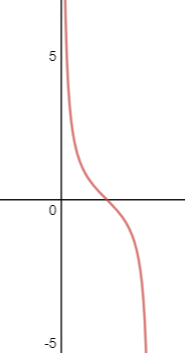
\includegraphics[width=0.3\textwidth]{./figures/4.png}
	\label{fig4}
\end{figure}

所以有
\begin{align*}
 	&(f)(1+f'^2) = (f)\big(1+\cot^2\frac{\theta}{2}\big) \\
 	&\hspace{5em} =
\end{align*}


\end{document}
